%!TEX root = main.tex
\author{Autor: Leonie Schiburr}
\section{Folgenethik}

Die Folgenethik, nachfolgend auch Utilitarismus genannt, beschäftigt sich mit der Suche nach der Maximierung des Glücks für
alle beteiligten Personen. Dabei wird zwischen den folgenden beiden ethischen Strömungen Unterschieden. Der Regelutilitarismus fragt nach der Handlung, die einer moralischen Regel entspricht und lehnt jede Handlung ab, die gegen eine moralische Regel verstößt. Der Handlungsutilitarismus sucht nach der Handlung, die für die meisten betroffenen Personen den größten Nutzen oder das größte Glück bringt.\\
\\
Betrachten wir die Dilemmasituation unseres Online-Dienstleisters Venus, stellt sich die Frage, ob es aus utilitaristischer Sicht ethisch ist,
unsere Dienstleistung nur für \glqq schöne\grqq~Menschen anzubieten.\\
\\
Zunächst sollte diese Frage aus der Sicht des Regelutilitarismus betrachtet werden. Bevor also eine Entscheidung darüber gefällt wird, welche Handlung den größtmöglichen Nutzen für die meisten Personen bringt, sollte Folgendes beantwortet werden:\\
\\
Widerspricht die Entscheidung, nur \glqq schönen\grqq~Menschen eine Mitgliedschaft zu gewähren, einer moralischen Regel?\\
\\
In diesem Fall lautet die Antwort \glqq Nein\grqq. Nun gibt es das Problem, dass Kindern bereits in sehr jungen Jahren beigebracht wird, andere Menschen nicht aufgrund des Aussehens, der Herkunft, der Religion oder einem anderen Grund auszugrenzen. Wie lässt sich begründen, dass die Handlung dennoch keiner moralischen Regel widerspricht? Im Fall des Online-Dienstes Venus handelt es sich um einen kostenpflichtigen, nicht öffentlichen Dienst, ähnlich einer Mitgliedschaft in einem \glqq Gentlemans Club\grqq. \\
Die Mitglieder zahlen für ihre Mitgliedschaft und es gibt Kriterien, die für eine erfolgreiche Bewerbung erfüllt werden müssen. Ähnliche Voraussetzungen gibt es auch bei der Beantragung eines Kredites bei einer Bank, oder der Bewerbung an einer privaten Hochschule.\\ 
\\
Einem Geschäft oder Unternehmen ist es gestattet, Kunden abzulehnen, die nicht ihren Vorstellungen entsprechen, da es sich um privaten Vertragsabschluss handelt, der nach deutschem Recht der Vertragsfreiheit als Bestandteil der allgemeinen Handlungsfreiheit unterliegt.\footnote{vgl. GG (2015), Art. 2 Abs. 1 GG} Zudem ist ein Kunde auf einen solchen Dienst, wie die Network-Plattform Venus, nicht angewiesen und hat die Wahl, sich nicht zu bewerben oder einen anderen Dienstleister in Anspruch zu nehmen. Dies jedoch beispielsweise auch für Schützenvereine, die sich weigern dürfen, Bürger einer bestimmten ethnischen Herkunft oder aufgrund sexueller Neigungen aufzunehmen, begründet im Allgemeinen Gleichstellungsgesetzt unter §20 \glqq Zulässige unterschiedliche Behandlung\grqq.\footnote{vgl. BGB (2015), § 20 AGG} Um die Antwort also aus ethischer Sicht genauer zu begründen, wird die eingehende Frage anders gestellt:\\
\\
Entspricht die Handlung einer moralischen Regel? Hier lautet die Antwort \glqq Ja\grqq.\\
\\
In diesem Fall können sogar mehrere moralischen Regeln betrachtet werden. Eine gesellschaftlich akzeptierte Regel lautet \glqq Sei Fair!\grqq. Um dieser moralischen Regel zu entsprechen, gewährleistet Venus, dass jede der möglichen Auswahlmethoden auf einem Verfahren beruht, das nicht durch den Anbieter oder andere beteiligte Personengruppen zu ihrem eigenen Vorteil beeinflusst werden kann. Eine weitere moralische Regel lautet \glqq Sei Ehrlich!\grqq. Um dies zu erreichen, werden alle möglichen Auswahlverfahren transparent gehalten. Zumindest soll die Möglichkeit für die Bewerber bestehen, einzelne Kriterien oder die Begründung für eine Ablehnung in Erfahrung bringen zu können. Zu guter Letzt gilt noch die Regel \glqq Sei Freundlich!\grqq. Alle Bewerber von Venus werden höflich und zuvorkommend behandelt und nicht in Kategorien eingeteilt, die sie beleidigen könnten.Social-Media-Plattformen, wie das Facebook für Schöne \glqq Beautiful People\grqq, lassen ihre Bewerber nach Kategorien wie \glqq absolutly not\grqq~oder \glqq mhm OK\grqq~einteilen. Eine Bewerbung bei Venus soll lediglich angenommen oder abgelehnt werden, ohne diese noch zu werten.\footnote{vgl. BeautifulPeople.com (2016), Online im Internet}\\
\\ 
Als nächstes stellt sich die Frage: Bringt die Entscheidung den größtmöglichen Nutzen für die meisten Beteiligten?\\
\\ 
Zur Klärung dieser Dilemmasituation muss jedoch zuerst festgelegt werden, ob und auf welche Art und Weise die Mitglieder ausgewählt werden sollen. Zudem ist wichtig, welche Stakeholder, also welche Parteien an der Entscheidung, nur \glqq Schöne\grqq~Menschen aufzunehmen, ein Interesse haben, oder von dieser betroffen sind. Für die Network-Plattform Venus wurden folgende Handlungsoptionen festgelegt:
\begin{itemize}
\item Alle Bewerber werden zugelassen, ob \glqq Schön\grqq~oder nicht.
\item Nur \glqq Schöne\grqq~werden zugelassen. Die Entscheidung, ob ein Mensch \glqq Schön\grqq~ist, soll durch einen Computeralgorithmus bestimmt werden. Die Kriterien, nach denen der Algorithmus entscheidet, werden öffentlich gemacht.
\item Nur \glqq Schöne\grqq~werden zugelassen. Die Entscheidung, ob ein Mensch \glqq Schön\grqq~ist, soll durch einen Computeralgorithmus bestimmt werden. Die Kriterien, nach denen der Algorithmus entscheidet, werden nicht veröffentlicht.
\item Nur \glqq Schöne\grqq~werden zugelassen. Die Entscheidung, ob ein Mensch \glqq Schön\grqq~ist, soll durch eine Jury aus bekannten Personen des öffentlichen Lebens (aus Politik, Wirtschaft, Mode usw.) bestimmt werden. Die Entscheidung der Jury ist subjektiv.
\item Nur \glqq Schöne\grqq~werden zugelassen. Die Entscheidung, ob ein Mensch \glqq Schön\grqq~ist, soll durch die eigenen Mitglieder bestimmt werden. Die Entscheidung der Community ist subjektiv.
\end{itemize}
Von der Entscheidung, die der Vorstand trifft, sind verschiedene Personengruppen betroffen. Neben den Entscheidungsträgern, hier dem Vorstand, sind auch noch die restlichen Mitarbeiter des Unternehmens betroffen. Eine Entscheidung für die ausschließliche Aufnahme von \glqq Schönen\grqq~Menschen, könnte für diese einen sozialen Druck bedeuten, da sie wohl möglich von anderen verurteilt werden, oder dich selbst für ihren Arbeitsplatz schämen. \glqq Schöne\grqq~Mitglieder haben gegebenenfalls ein Interesse daran, zu einem elitären Club zu gehören und würden mit der Entscheidung, jedem die Mitgliedschaft zu gewähren, nicht einverstanden sein. \glqq Hässliche\grqq~Menschen könnten sich durch die ausschließliche Aufnahme von \glqq Schönen\grqq~Menschen gekränkt fühlen. Die Investoren haben ein Interesse daran, dass das Unternehmen sich am Markt etabliert und hohe Gewinne erzielt. Andererseits möchten die Investoren ihren Ruf nicht durch ein schlechtes Image, wie \glqq Oberflächlichkeit\grqq, schädigen.

Um zu ermitteln welche der Handlungsoptionen den größtmöglichen Nutzen bringt, wird eine Tabelle mit allen Stakeholdern angefertigt. Anschließend werden den Handlungsoptionen
für jeden Stakeholder Zahlen zugewiesen, die den Nutzen bzw. Schaden, den ein Stakeholder von einer Handlung erfährt, widerspiegelt. Nach der Betrachtung aller Sichtweisen ergibt sich folgende Ergebnistabelle:
\begin{figure}[hbt]
	\centering
	\begin{minipage}[t]{1\textwidth} % Breite, z.B. 1\textwidth		
	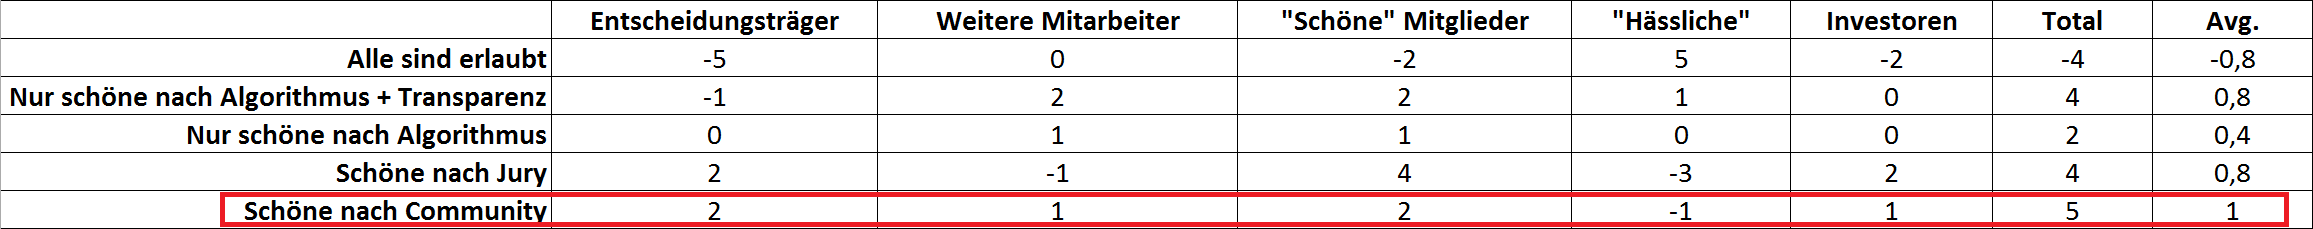
\includegraphics[width=1\textwidth]{Handlungsutilitarismus.png}\\ % Pfad
	%\source{Eigene Darstellung} % Quelle
	\caption{Matrix Handlungsutilitarismus} % Überschrift
	\label{abb:util}
	\end{minipage}
\end{figure}

Aus der Tabelle ergibt sich, dass die Handlungsoption \glqq Schöne nach Community\grqq~für die meisten betroffenen Personen den größtmöglichen Nutzen bringt. Für \glqq Schöne\grqq~Menschen bleibt bei dieser Form der Auswahl die Online-Plattform eine elitäre Einrichtung. Zudem dürfen Mitglieder über die Aufnahme der Bewerber entscheiden. Dadurch, dass die Aufnahme den Mitgliedern vorbehalten ist, hat das Unternehmen keinen Einfluss auf das Verfahren. Somit bleiben die Mitarbeiter und Investoren von möglichen Vorwürfen weitestgehend verschont. Zwar bedeutet die Wahl durch die Community weniger Prestige als beispielsweise die Auswahl aurch eine prominente Jury, doch profitieren das Unternehmen und die Investoren davon, dass sich das Portal als Marke etablieren und so potentiell mehr Gewinn erzielt werden kann.

Nach der Aufschlüsselung der Dilemmasituation aus Sicht des Utilitarismus kann abschließend folgendes Fazit gezogen werden: Die Entscheidung, Venus nur für \glqq Schöne\grqq~Menschen zu öffnen, ist nach einer Analyse aus regel- und handlungsutilitaristischer Sicht ethisch. 



% Sokrates
